
\documentclass[
	10pt,aspectratio=169 % Set the default font size, options include: 8pt, 9pt, 10pt, 11pt, 12pt, 14pt, 17pt, 20pt
	%t, % Uncomment to vertically align all slide content to the top of the slide, rather than the default centered
	%aspectratio=169, % Uncomment to set the aspect ratio to a 16:9 ratio which matches the aspect ratio of 1080p and 4K screens and projectors
]{beamer}


\usepackage{listings}
\usepackage{xcolor}

%\graphicspath{{Images/}{./}} % Specifies where to look for included images (trailing slash required)
\usepackage{booktabs} 
%----------------------------------------------------------------------------------------
%	SELECT LAYOUT THEME
%----------------------------------------------------------------------------------------

% Beamer comes with a number of default layout themes which change the colors and layouts of slides. Below is a list of all themes available, uncomment each in turn to see what they look like.

%\usetheme{default}
%\usetheme{AnnArbor}
%\usetheme{Antibes}
%\usetheme{Bergen}
%\usetheme{Berkeley}
%\usetheme{Berlin}
%\usetheme{Boadilla}
%\usetheme{CambridgeUS}
%\usetheme{Copenhagen}
%\usetheme{Darmstadt}
%\usetheme{Dresden}
%\usetheme{Frankfurt}
%\usetheme{Goettingen}
%\usetheme{Hannover}
%\usetheme{Ilmenau}
%\usetheme{JuanLesPins}
%\usetheme{Luebeck}
\usetheme{Madrid}
%\usetheme{Malmoe}
%\usetheme{Marburg}
%\usetheme{Montpellier}
%\usetheme{PaloAlto}
%\usetheme{Pittsburgh}
%\usetheme{Rochester}
%\usetheme{Singapore}
%\usetheme{Szeged}
%\usetheme{Warsaw}

    %%%%%%%%%%%%
    %% COLORS %%
    %%%%%%%%%%%%

%\usecolortheme{albatross}
%\usecolortheme{beaver}
%\usecolortheme{beetle}
%\usecolortheme{crane}
%\usecolortheme{dolphin}
%\usecolortheme{dove}
%\usecolortheme{fly}
%\usecolortheme{lily}
%\usecolortheme{monarca}
%\usecolortheme{seagull}
%\usecolortheme{seahorse}
%\usecolortheme{spruce}
%\usecolortheme{whale}
%\usecolortheme{wolverine}


\setbeamertemplate{blocks}[rounded][shadow=false]
\usefonttheme{default} % Typeset using the default sans serif font
\usefonttheme{serif} % Typeset using the default serif font (make sure a sans font isn't being set as the default font if you use this option!)
%\usefonttheme{structurebold} % Typeset important structure text (titles, headlines, footlines, sidebar, etc) in bold
%\usefonttheme{structureitalicserif} % Typeset important structure text (titles, headlines, footlines, sidebar, etc) in italic serif
%\usefonttheme{structuresmallcapsserif} % Typeset important structure text (titles, headlines, footlines, sidebar, etc) in small caps serif



%------------------------------------------------

%\usepackage{mathptmx} % Use the Times font for serif text
\usepackage{palatino} % Use the Palatino font for serif text
\usepackage{listings}
%\usepackage{helvet} % Use the Helvetica font for sans serif text
\usepackage[default]{opensans} % Use the Open Sans font for sans serif text
\usepackage{ragged2e}
%\usepackage[default]{FiraSans} % Use the Fira Sans font for sans serif text
%\usepackage[default]{lato} % Use the Lato font for sans serif text

%----------------------------------------------------------------------------------------
%	SELECT INNER THEME
%----------------------------------------------------------------------------------------

%\useinnertheme{default}
%\useinnertheme{circles}
%\useinnertheme{rectangles}
\useinnertheme{rounded}
%\useinnertheme{inmargin}

%\useoutertheme{default}
%\useoutertheme{infolines}
%\useoutertheme{miniframes}
%\useoutertheme{smoothbars}
%\useoutertheme{sidebar}
%\useoutertheme{split}
%\useoutertheme{shadow}
%\useoutertheme{tree}
%\useoutertheme{smoothtree}

%\useinnertheme{rectangles}                                                                                                    
\usefonttheme{professionalfonts}                                  \usecolortheme{structure}                                         \usepackage{times} 


%\setbeamertemplate{footline} % Uncomment this line to remove the footer line in all slides
%\setbeamertemplate{footline}[page number] % Uncomment this line to replace the footer line in all slides with a simple slide count

%\setbeamertemplate{navigation symbols}{} % Uncomment this line to remove the navigation symbols from the bottom of all slides

%----------------------------------------------------------------------------------------
%	PRESENTATION INFORMATION
%----------------------------------------------------------------------------------------

\title[Remarks on the Numerical Analysis ...]{Remarks on the Numerical analysis of basins of attraction using complex variables} % The short title in the optional parameter appears at the bottom of every slide, the full title in the main parameter is only on the title page

\subtitle{} % Presentation subtitle, remove this command if a subtitle isn't required

\author[Ribeiro, M. A.]{Mauricio A. Ribeiro, Pamela R. Martins, Hilson H. Daum, Ângelo M. Tusset, Jose M. Balthazar} % Presenter name(s), the optional parameter can contain a shortened version to appear on the bottom of every slide, while the main parameter will appear on the title slide


\institute[UTFPR-PG]{ \\ \smallskip 
PPGEE - UTPFR, DeFis – PUC, PPGEP – UTFPR, PPGEP – UTFPR,  PPGEP – UTFPR, FEB-UNESP-Bauru \\ \smallskip 
\textit{mau.ap.ribeiro@gmail.com}} % Your institution, the optional parameter can be used for the institution shorthand and will appear on the bottom of every slide after author names, while the required parameter is used on the title slide and can include your email address or additional information on separate lines

\date[mau.ap.ribeiro@gmail.com]{\tiny{IV CONFERENCE ON DYNAMICS, CONTROL, AND APPLICATIONS TO APPLIED ENGINEERING AND LIFE SCIENCE AND} \\
\tiny{I WORKSHOP ON NONLINEAR DYNAMICS, ENERGY PRODUCTION, RENEWABLE ENERGY SOURCES, ENERGY TRANSFER AND ENERGY HARVESTING}} % Presentation date or conference/meeting name, the optional parameter can contain a shortened version to appear on the bottom of every slide, while the required parameter value is output to the title slide

%----------------------------------------------------------------------------------------

\pgfdeclareimage[height=1.5cm]{logo}{Dycaels}
\logo{\pgfuseimage{logo}}
\setbeamercovered{transparent} 
\setbeamercolor{structure}{fg=red!60!black}
\begin{document}

%----------------------------------------------------------------------------------------
%	TITLE SLIDE
%----------------------------------------------------------------------------------------

\begin{frame}
	\titlepage 
\end{frame}

\begin{frame}{Outline}
    \transwipe
    \tableofcontents
\end{frame}
\section{Introduction}
\begin{frame}{Introduction}
    \transwipe
    \begin{itemize}
        \item If we consider complex variables ($z \in \mathbb{C}$)
         \item Chaotic systems with real variables are widely studied.
         \item Chaotic systems with complex variables is a more recent issue for nonlinear dynamic analysis
         \item Its applications range from: physics, quantum mechanics, astrophysics, dynamics of high energy accelerators, etc. \footnote{Marshall, Delmar, and J. C. Sprott. "Simple driven chaotic oscillators with complex variables." Chaos: An Interdisciplinary Journal of Nonlinear Science 19.1 (2009).} \footnote{Mahmoud, G.M., Mahmoud, E.E. Phase and antiphase synchronization of two identical hyperchaotic complex nonlinear systems. Nonlinear Dyn 61, 141–152 (2010).}.
    \end{itemize}
\end{frame}
\section{Mathematical Modeling}
\begin{frame}{Mathematical Modeling}
    \transwipe
    \begin{itemize}
        \item Considering the variables $z \in \mathbb{c}$ described by $z=x+yi$, $\dot{z}=\dot{x}+i\dot{y}$ and $\bar{z}=x-yi$, therefore, an oscillator can be described as follows:
        \begin{equation}
        \dot{z}+f(z,\bar{z})=A\rm{e}^{i \omega t}
        \label{eq:01}
        \end{equation}
\item In this way, rewriting Eq. \ref{eq:01}, we have:
\begin{eqnarray}
\dot{x} &=& -\Re(f(z,\bar{z}))+Acos(\omega t) \\ \nonumber
\dot{y} &=& -\Im(f(z,\bar{z}))+Asin(\omega t) \\ \nonumber
\end{eqnarray}
\item Whereas:
\begin{equation}
    f(z,\bar{z})=(z^2-\bar{z}^2)z+\bar{z}
\end{equation}
\end{itemize}
Therefore, we have:
\begin{eqnarray}
    \dot{x} &=& 4xy^2 -x+ A cos(\omega t) \\ \nonumber
    \dot{y} &=& -4x^2y -y+ A sin(\omega t)
\end{eqnarray}
\end{frame}

\begin{frame}{Coefficient of uncertainty and entropy of basins of attraction}
    \transwipe
    \begin{block}{Uncertainty Coefficient}
    \begin{itemize}
    \item This is related to the sensitivity of the final state of the phase space trajectories.
    \begin{itemize}
    \item An exponent close to $1$ means that the basin of attraction has smooth contours;
     \item An exponent close to $0$ means that the attraction basin is fractalized (sieved attraction basins).
    \end{itemize}
    \item The uncertainty coefficient defines the uncertainty of the initial conditions of the system, which can be attracted by two or more attractors.
    \end{itemize}
    \end{block}
\end{frame}

\begin{frame}{Uncertainty Coefficient and entropy of basins of attraction}
    \framesubtitle{Entropy Basins of Attraction}
        \begin{itemize}
        \item A measure to quantify the uncertainty of basins of attraction;
         \item Provides an efficient condition for the existence of fractal limits, when the entropy is greater than $log(2)$ the basin is fractal;
         \item The basin of attraction is considered with a phase space coloring where each initial condition corresponds to a color referring to an attractor\footnotemark[1].
         \item To calculate entropy, we define a ball of radius $\varepsilon$, the proportion of the colors of each ball $\varepsilon$ defines the probability $P_j$ associated with each color\footnotemark[2]. The entropy of basins of attraction is defined as the mean Gibbs entropy $(S_i)$ which is given by:
            \begin{equation}
                S_i = -\sum^{N_a}_{j=1}P_jlog(P_j)
            \end{equation}
     Where $N_a$ is the number of different colors of the attraction basin,
        \end{itemize}

    \footnotemark[1]{\tiny{Daza, A., Wagemakers, A., \& Sanjuán, M. A. (2022). Classifying basins of attraction using the basin entropy. Chaos, Solitons \& Fractals, 159, 112112.}}\\
    \footnotemark[2]{\tiny{Daza, Alvar, et al. "Basin entropy: a new tool to analyze uncertainty in dynamical systems." Scientific reports 6.1 (2016): 31416.}}
\end{frame}

\section{Numerical Results}
\begin{frame}{Numerical Results}
   \transwipe
   \begin{columns}
   \column{0.5\textwidth}
   
    \begin{itemize}
        \item For numerical analyzes we used the 4th order Runge and Kutta method, with an integration step $h=0.001$ and a total time of $10^6[s]$
         \item The transient time of $40\%$ of the total time;
         \item $\omega = 1.0$
         \item $A\in [0.5, 1.0]$
         \item Attraction basins a grid $x^{0} \in [-1,1] \times y^0 \in [-1,1]$ of $800\times 800$ points; 
        

    \end{itemize}
    \column{0.5\textwidth}
    \begin{block}{Mathematical Modeling}
        \begin{eqnarray}
           \dot{x} &=& 4xy^2 -x+ A cos(\omega t) \\ \nonumber
           \dot{y} &=& -4x^2y -y+ A sin(\omega t)
        \end{eqnarray}
        \end{block}
   \end{columns}
   
\end{frame}


\begin{frame}{Numerical Results}
    \begin{figure}
        \centering
        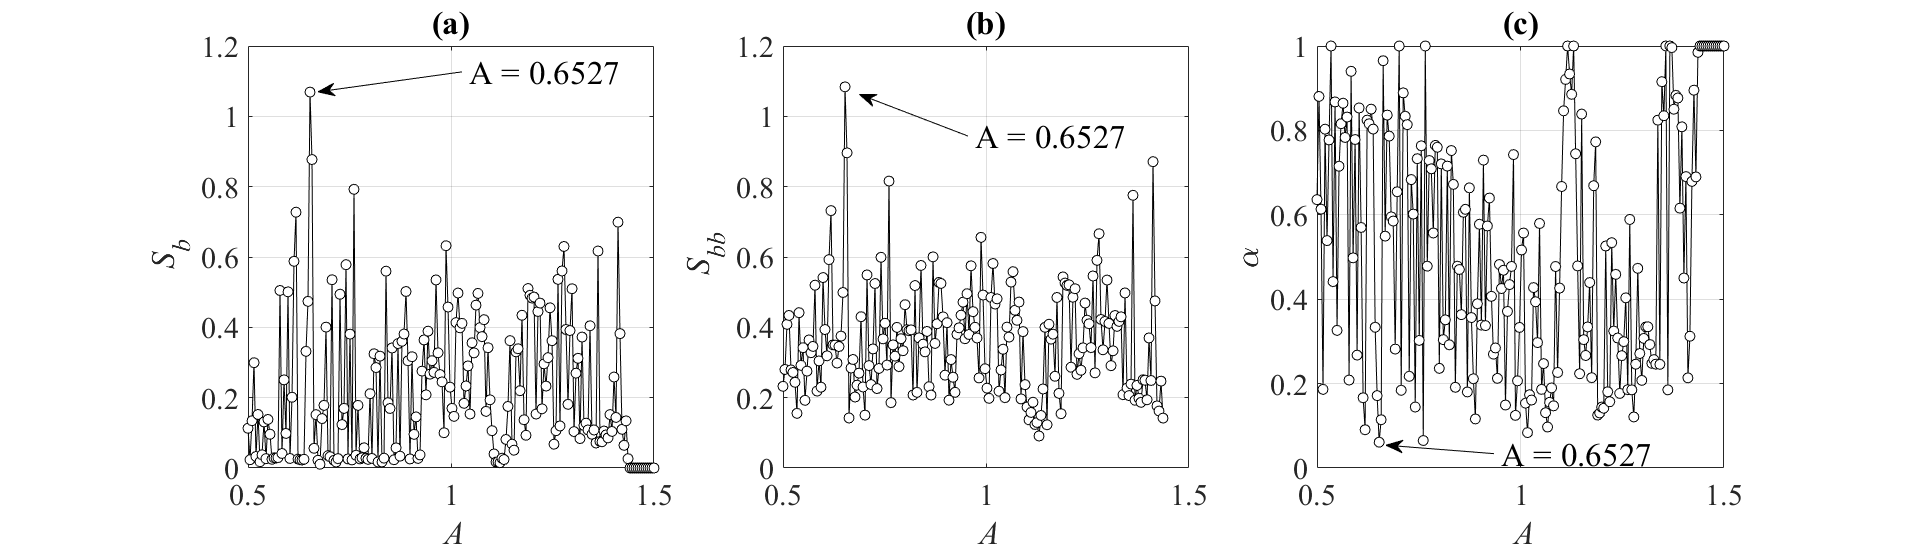
\includegraphics[scale=0.30]{Imagens/entropia_alfa.png}
        \caption{(a) Entropy basin, (b) Entropy basin boundery and (c) uncertain coefficient. }
        \label{fig:fig01}
    \end{figure}
\end{frame}

\begin{frame}{Numerical Results}
   \transwipe
\begin{columns}
\column{0.6\textwidth}
    \begin{figure}
        \centering
        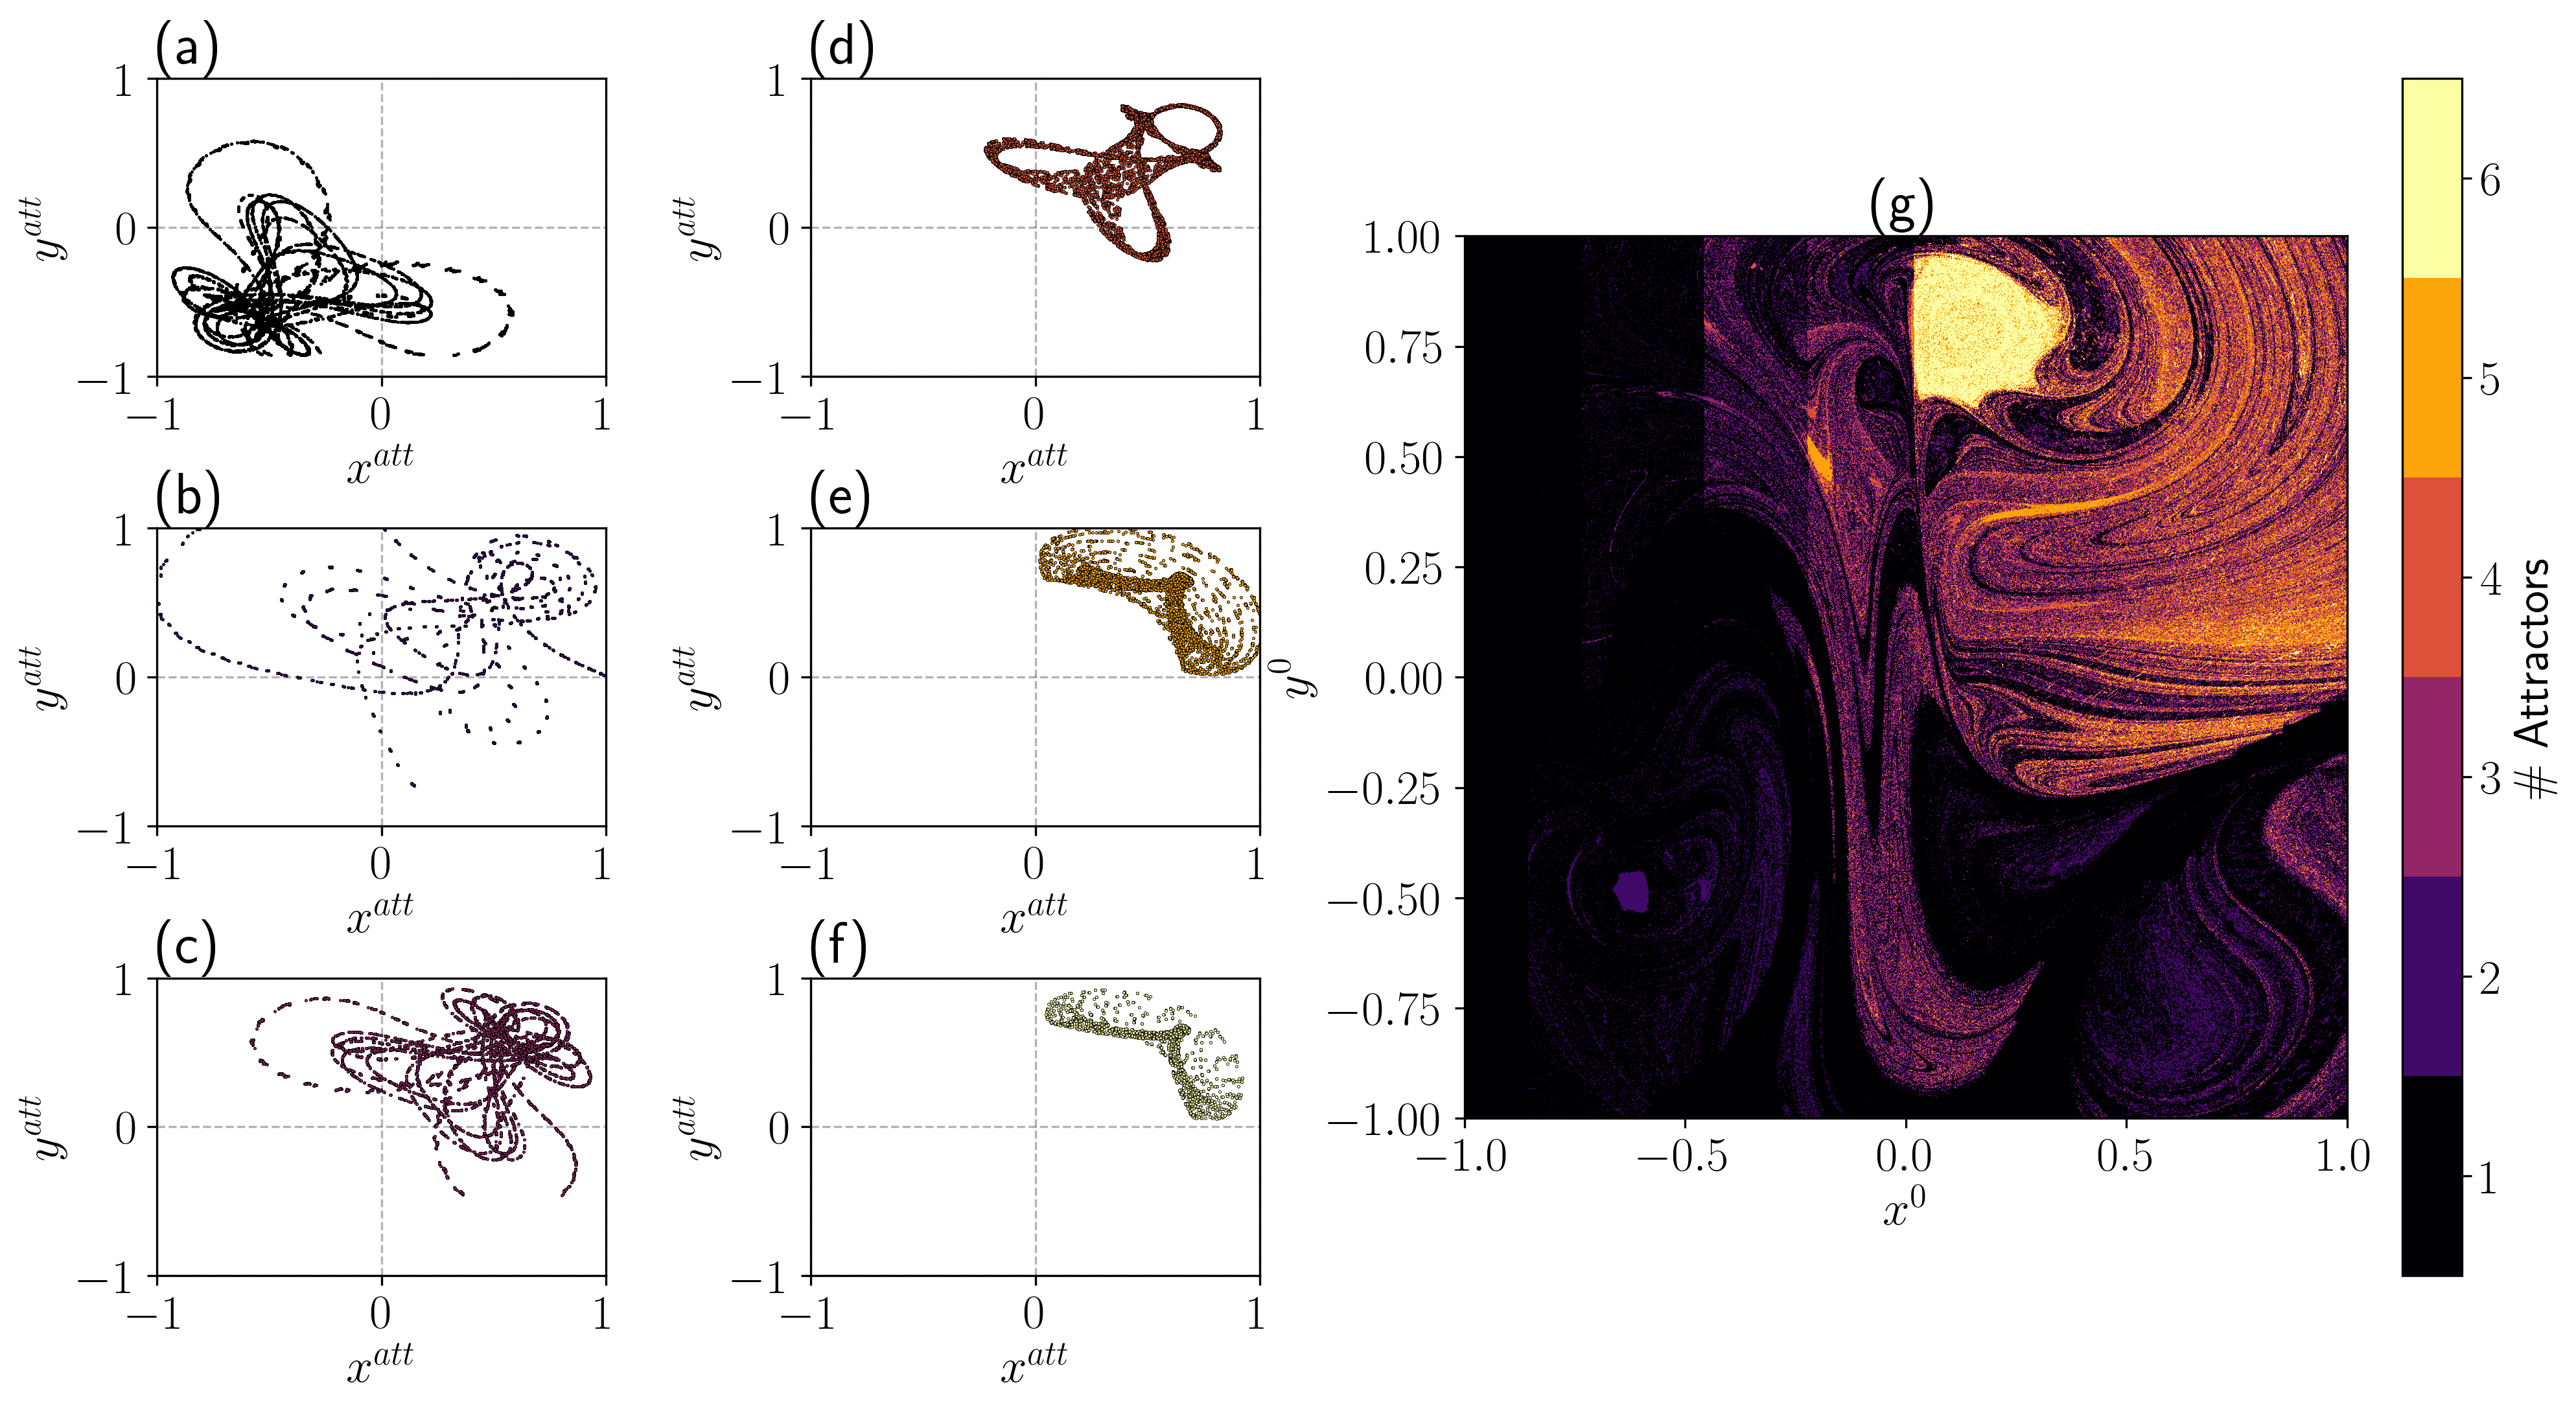
\includegraphics[scale=0.27]{Imagens/basins.png}
        \caption{(a)-(f) attractors e (g) Basin of attraction.}
        \label{fig:fig02}
    \end{figure}
\column{0.4\textwidth}
\begin{itemize}
\item For $A = 0.6527$ the entropy of the attraction basins and the edge are maximum, with $A = 0.6527 > log(2)$ the attraction basin has a fractal behavior
\item Containing $6$ represented in fig. \ref{fig:fig02} (a)-(f) attractors, with $S_{b} = 1.069 $, $S_{bb} = 1.084 $ and $ \alpha = 0.061$.
\end{itemize}
\end{columns}    
\end{frame}

\begin{frame}{Numerical Results}
   \transwipe
\begin{columns}
\column{0.5\textwidth}
    \begin{figure}
    \centering
    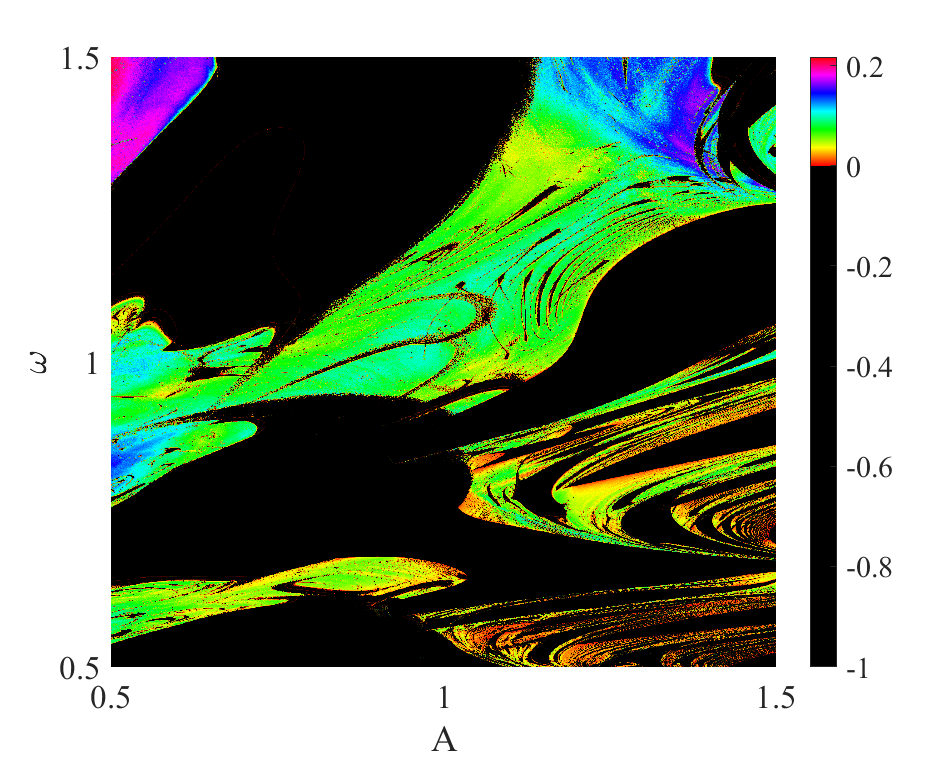
\includegraphics[scale=0.3]{Imagens/Lyapunov2D.png}
    \caption{Lyapunov Exponent for $A \in [0.5, 1.0] \times \omega \in [0.5, 1.0]$}
    \label{fig:fig03}
    \end{figure} 
    \column{0.5\textwidth}
    \begin{itemize}
    \item Considering the initial condition $(0,0)$ we calculate the Lyapunov Exponent $(\lambda)$ considering the following intervals $\omega \in [0.5,1.0] \times A \in[0.5, 1.0]$
         \item Region in black $(\lambda<0)$ regions in which the system has orbits with periodic behavior.
         \item Region between xxx and red $(\lambda>0)$ region in which the system has orbits with chaotic behavior.
    \end{itemize}
\end{columns}
\end{frame}

\begin{frame}{Numerical Results}
   \transwipe
    \begin{columns}
        \column{0.5\textwidth}
        \begin{figure}
            \centering
            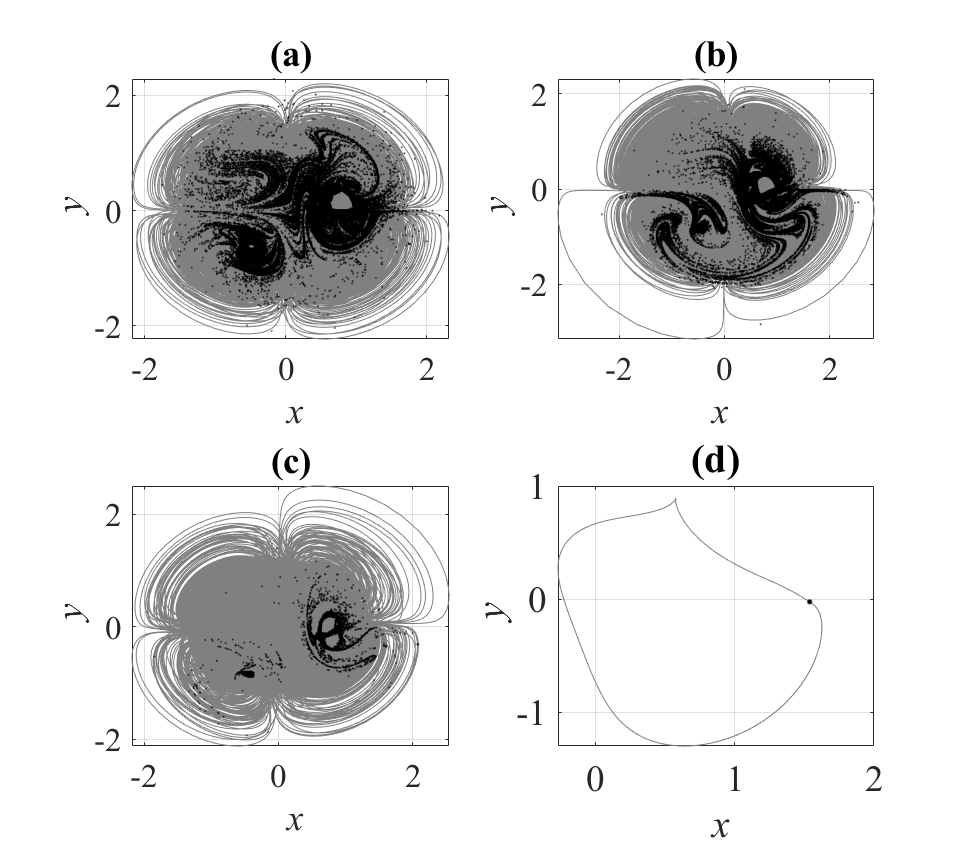
\includegraphics[scale=0.25]{Imagens/mapadefasenovo.png}
            \caption{ Phase maps (Gray line) and Poincare maps (Black dots for$\omega=1.0$. (a)$A=0.6527$,(b) $A=1.0$,(c) $A=1.1$ and (d) $A=1.3$}
            \label{fig:04}
        \end{figure}
        \column{0.5\textwidth}
        \begin{itemize}
            \item (a) $A=0.6527$, chaotic behavior
            \item (b) $A=1.0$,  chaotic behavior
            \item (c) $A=1.1$,  chaotic behavior
            \item (d) $A=1.3$,  periodic behavior.
        \end{itemize}
    \end{columns}
\end{frame}
\section{Conclusion}

\begin{frame}{Conclusion}
     \transwipe
   \begin{itemize}
\item The use of the entropy of attraction basins and the uncertainty coefficient corroborates the determination of attraction basins with screening in oscillatory systems in complex variables.
        \item Such analyzes also allow determining the behavior of attraction basins in electromechanical systems.
        \item The dynamic analyzes with the Maximum Lyapunov Exponent $(\lambda)$ are the regions for the parametric analysis $(A \times \omega)$ the chaos regions and the periodic regions.
        \item Phase and Poincaré Maps showed the behavior of trajectories in phase space.
        \item For future work, determine the parameter space for entropy and the uncertainty coefficient to determine the sieve regions of the attraction basins.
   \end{itemize}  
\end{frame}

   
\section{References}
   \transwipe
\begin{frame}{References}
    \begin{enumerate}
        \item Daza, Alvar, et al. "Basin entropy: a new tool to analyze uncertainty in dynamical systems." Scientific reports 6.1 (2016): 31416.
        \item Daza, Alvar, Alexandre Wagemakers, and Miguel AF Sanjuán. "Classifying basins of attraction using the basin entropy." Chaos, Solitons and Fractals 159 (2022): 112112.
        \item Puy, Andreu, et al. "A test for fractal boundaries based on the basin entropy." Communications in Nonlinear Science and Numerical Simulation 95 (2021): 105588. 
        \item Grebogi, Celso, et al. "Final state sensitivity: an obstruction to predictability." Physics Letters A 99.9 (1983): 415-418.
        \item McDonald, Steven W., et al. "Fractal basin boundaries." Physica D: Nonlinear Phenomena 17.2 (1985): 125-153.
    \end{enumerate}
\end{frame}

\end{document} 
